\documentclass[11pt]{article}
\usepackage{geometry}                
\geometry{letterpaper}                   

\usepackage{graphicx}
\usepackage{amssymb}
\usepackage{epstopdf}
\usepackage{natbib}
\usepackage{verbatim}
\usepackage{amssymb, amsmath}
\usepackage[numbered, framed]{mcode}
\DeclareGraphicsRule{.tif}{png}{.png}{`convert #1 `dirname #1`/`basename #1 .tif`.png}

%\title{Title}
%\author{Simon Schmid, Daniel Z\"und}
%\date{\today} 

\begin{document}



\thispagestyle{empty}

\begin{center}

\includegraphics[width=5cm]{ETHlogo.eps}

\bigskip


\bigskip


\bigskip


\LARGE{ 	Lecture with Computer Exercises:\\ }
\LARGE{ Modelling and Simulating Social Systems with MATLAB\\}

\bigskip

\bigskip

\small{Project Report}\\

\bigskip

\bigskip

\bigskip

\bigskip


\begin{tabular}{|c|}
\hline
\\
\textbf{\LARGE{Evacuation Bottleneck}}\\
\\
\hline
\end{tabular}
\bigskip

\bigskip

\bigskip

\LARGE{Daniel Z\"und \& Simon Schmid}



\bigskip

\bigskip

\bigskip

\bigskip

\bigskip

\bigskip

\bigskip

\bigskip

Z\"urich\\
May 2010\\

\end{center}



\newpage

%%%%%%%%%% Agreement n�1 %%%%%%%%%%%%%%%%%
\section*{Eigenst\"andigkeitserkl\"arung}
\bigskip



\bigskip


\large
Hiermit erkl\"are ich, dass ich diese Gruppenarbeit selbst\"andig verfasst habe,
keine anderen als die angegebenen Quellen-Hilsmittel verwenden habe, und alle
Stellen, die w\"ortlich oder sinngem\"ass aus ver\"offentlichen Schriften entnommen
wurden, als solche kenntlich gemacht habe. Dar\"uber hinaus erkl\"are ich, dass 
diese Gruppenarbeit nicht, auch nicht auszugsweise, bereits f\"ur andere Pr\"ufung
ausgefertigt wurde.

\begin{center}

\bigskip


\bigskip


\begin{tabular}{@{}p{3.3cm}@{}p{6cm}@{}@{}p{6cm}@{}}
\begin{minipage}{3cm}

\end{minipage}
&
\begin{minipage}{6cm}
\vspace{2mm} \large Daniel Z\"und

 \vspace{\baselineskip}

\end{minipage}
&
\begin{minipage}{6cm}

\large Simon Schmid

\end{minipage}
\end{tabular}


\end{center}


%%%%%%%%%%%%%%%%%%%%%%%%%%%%%%%%%%%%%%%
%%%%%%%%%% Agreement n�2 %%%%%%%%%%%%%%%%%

\newpage
\section*{Agreement for free-download}
\bigskip


\bigskip


\large We hereby agree to make our source code for this project freely available for download from the web pages of the SOMS chair. Furthermore, we assure that all source code is written by ourselves and is not violating any copyright restrictions.

\begin{center}

\bigskip


\bigskip


\begin{tabular}{@{}p{3.3cm}@{}p{6cm}@{}@{}p{6cm}@{}}
\begin{minipage}{3cm}

\end{minipage}
&
\begin{minipage}{6cm}
\vspace{2mm} \large Daniel Z\"und

 \vspace{\baselineskip}

\end{minipage}
&
\begin{minipage}{6cm}

\large Simon Schmid

\end{minipage}
\end{tabular}


\end{center}
\newpage

%%%%%%%%%%%%%%%%%%%%%%%%%%%%%%%%%%%%%%%

 


%%%%%%%%%% Table of content %%%%%%%%%%%%%%%%%

\tableofcontents

\newpage

%%%%%%%%%%%%%%%%%%%%%%%%%%%%%%%%%%%%%%%





\section{Individual contributions}
For the implementation, Daniel Z\"und did most of the continuous model and
Simon Schmid implemented most of the best response dynamics.
The report was a teamwork of both, both wrote, reviewed each other and
corrected it.


\newpage
\section{Introduction and Motivations} 
People tend to form a crowd in states of emergency. The typical flight
behaviour is moving away from the source of danger. In open space people would
diffuse in all directions but if there are boundaries like walls or a street
the only way out is an exit. Usually, exits are small in comparison to the
crowd so the flow of people through the exit will be larger than the exit's
capacity. The result manifests itself as a bottleneck. The typical appearance
of a bottleneck is a semi-circular crowd around the exit. The main objective
of every evacuation plan is a sufficient amount of exits which are well
distributed so that the crowd splits up in smaller crowds. The interesting
point here is that the crowd will not spread evenly because of the individual and
collective behaviour of human beings.  People tend to head towards known and
visible exits which aren't crowded. This preference for a specific exit may
change depending on the circumstances. Our simulation is focused on how people
chose an exit and how this decision affects the collective behaviour.

\newpage
\section{Description of the Model}
\subsection{Model Overview} 

This section is a brief description of the model we implemented. We have
chosen a continous model for our simulation. The benefit of a continuous
simulation is that infinitesimal movements are possible and we think, it
shows the movement of people in a more natural way. 

The room is a two dimensional space, which includes three different types of
agents. The first are the people, which need to be evacuated, and the second
are the wall elements. The third kind are the door agents, which define a door.
The big difference between the three kinds, is that the door and wall
agents can not move.
The agents on the other side, need to move, so that they can get out of the
room. They move according to potentials, in whose radius they are. Since we
are working with potential fields, the agents want to go into the direction of
the negative gradient of the sum of all fields. This is mathematically
described as:

\[ m\frac{\delta^2 x_p}{\delta t^2}  = - \sum^{N}_{q = 1, q \neq p}
\nabla_{x_p} V_{agent}(|x_p - x_q|) - \nabla_{x_p} V_{door}(|x_p - x_q|) 
- \sum^{W}_{q = 1} \nabla_{x_p} V_{wall}(|x_p - x_q|)\]
where
\begin{itemize}
	\item $V_{agent}$ \ldots potential-field of other people.	
	\item $V_{wall}$ \ldots potential-field of wall elements.
	\item $V_{door}$ \ldots potential-field of the door, an agent is heading
	for.
\end{itemize}
Since the wall and door elements do not move, they build a static field
together. The dynamic part of the field comes from the moving people.
Each person in the room induces a field, that repels the other agents. So this
one has a strong influence on how the people move in the room.
In other words, the doors and walls introduce a static field on the whole
room, and the people a dynamic field. This allows us to simulate realistic
escape dynamics.

The model is chosen according to a homework from the lecture \textit{Simulations
using Particles} by Prof. Petros Koumoutsakos.

It is known, that people try to follow each others, as long as there is a
constant flow. Once the flow stagnates, it is a matter of patience before
people start to panic. In this situation people push each other towards the
exit, trying to get out of the room. Instead of moving on faster this
behaviour will cause clogging. If this happens people on the margin of the
crowd will perhaps reconsider their decision an move away from the crowded
exit to an uncrowded one, even if the door was familiar to them. In conclusion
this means people will follow only moving people.

In our model, the people choose their door according to some game theoretical
approach \cite{BestResponseDynamics}. The agents will calculate the opportunity costs of each exit by
weighting the queue in front of the door, the distance to the door and
individual preference factors like familiarity and visibility of the door. The
individual preference factors and velocities are distributed randomly on
initialization.

\subsection{Wall Potentials} 

The simulation takes the natural behaviour of
avoiding to walk close to walls into account by using repulsive wall
potentials inversely proportional to the distance from the walls. 
Actually the walls are formed by a row of fixed agents. 
\[V_{wall}(r) = k_W  \frac{1}{r}\]
The range of the wall effect is restricted up to the distance $D_{max}$ from
the walls. This prevents taking a wall into account which is on the other side
of the room. $k_W$ is a constant, which describes, how strong the repulsive 
force of the wall is.

\subsection{Door Potentials}
The door potentials behave almost like the wall potential, the big difference
here is, that they are attracting. This means that they are proportional to
the square of the distance an agent is away from it.
\[V_{door}(r) = k_D (r + s)^2\]
$k_D$ is another constant describing the strength of the attracting force
caused by the door. The shifting $s$ factor is needed because the potential
mentioned above would have a zero gradient if the radius is zero. The door is
formed by a row of door agents which are uniformly distributed on the door's
width.

\subsection{People Potentials}
The potentials of the people is pretty much like the potential of the walls.
It also repels people, which are close.
\[V_{agent}(r) = k_A  \frac{1}{r}\]
What we used in our simulation is that the agents have an other constant $k_A$
in front of the $\frac{1}{r}$.

\subsection{Potential field}
All the various potentials result in a single force which acts on the agent.
The agent reacts according to this field and moves, as mentiond
above, along the negative gradient of the sum of all potentials.
The following pictures show how the static part of a room may look
like. The figure \ref{emptyRoom} illustrates an empty room. The static field of
this figure looks like the plots shown in figure \ref{contour} and \ref{3D}.
For these plots, the field was calculated, as if an agent was
heading for the door which is on the west side of the room \footnote{The plots
are limited to a maximum value of 2500. Otherwise the values could go up to 
infinity, if we hit a wall element exactly. In that case, we would not see
anything of the rest, just a plain area.}.
\begin{figure}
	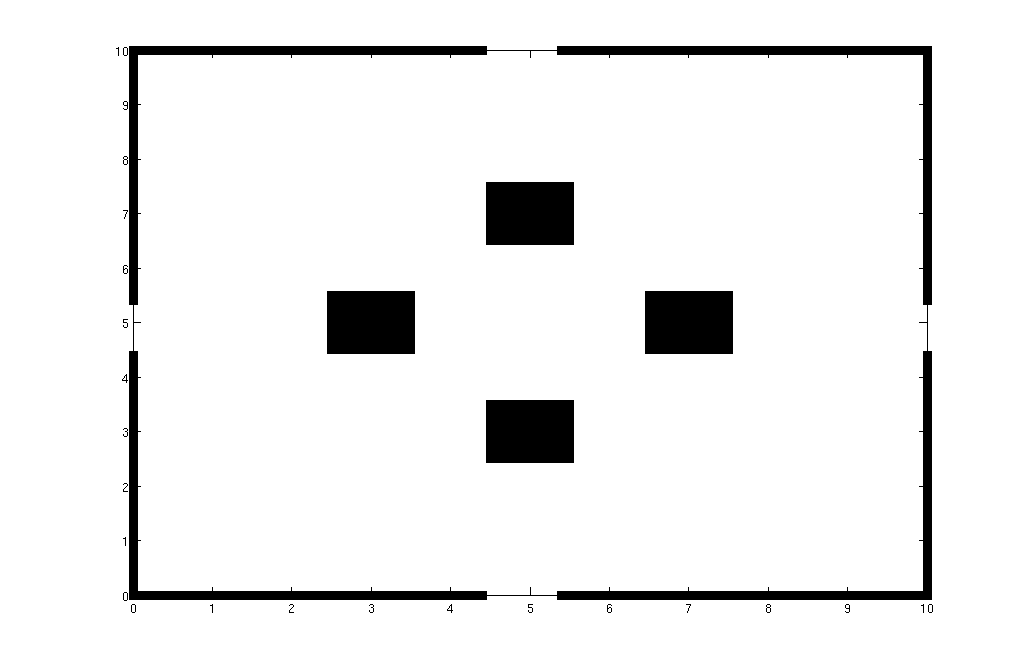
\includegraphics[width=\textwidth]{../graphen/emptyRoom.png}
	\caption{An example of an empty room}
	\label{emptyRoom}
\end{figure}
\begin{figure}
	\centering
	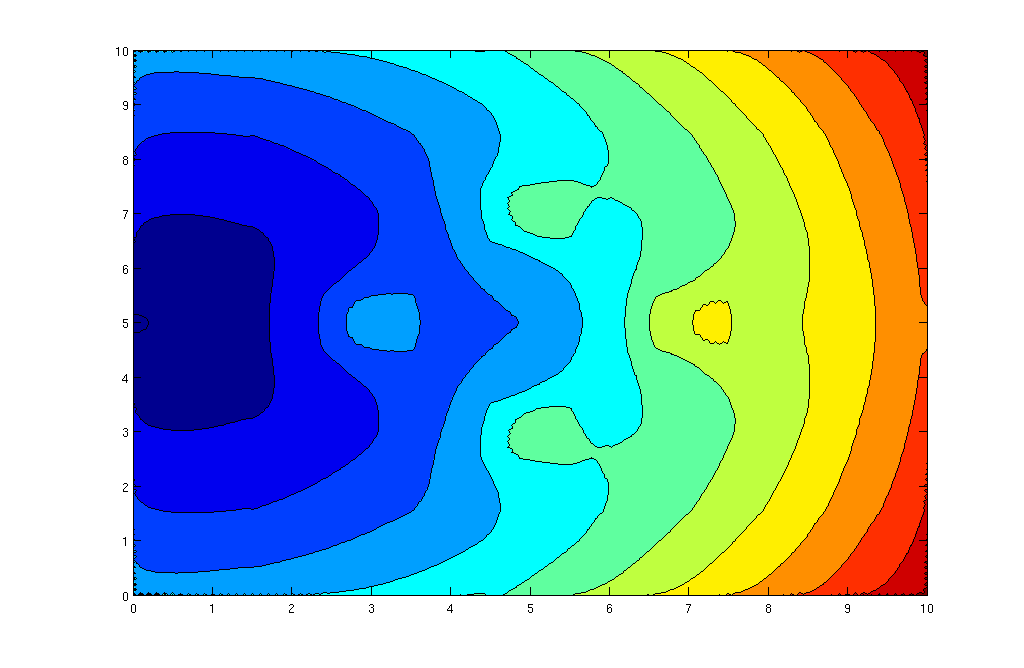
\includegraphics[width=0.8\textwidth]{../graphen/contour.png}
	\caption{Contour plot of room in figure \ref{emptyRoom}}
	\label{contour}
\end{figure}
\begin{figure}
	\centering
	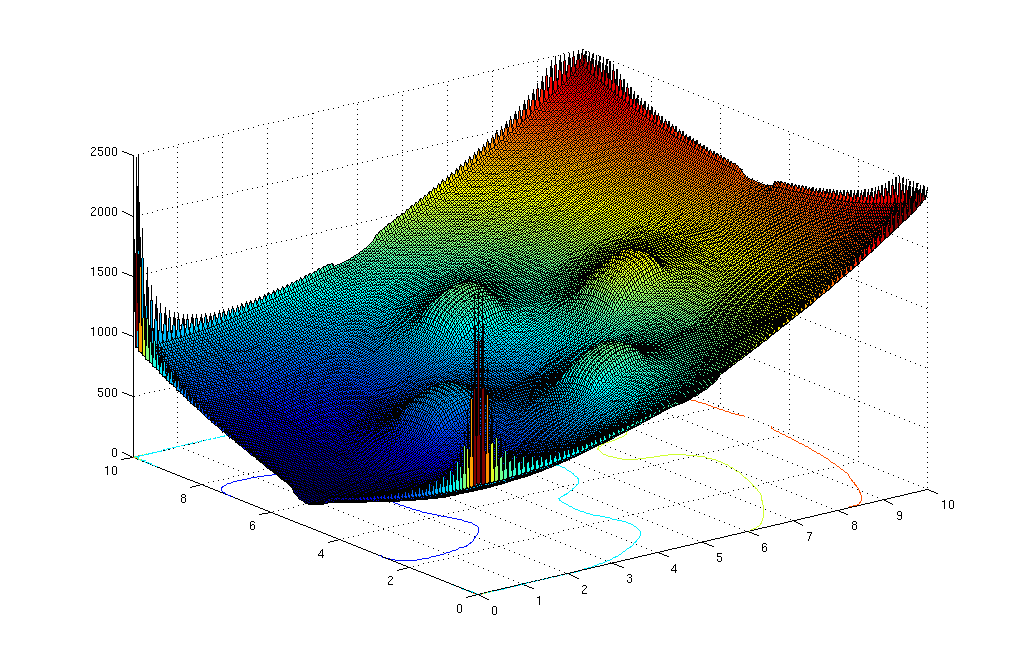
\includegraphics[width=0.8\textwidth]{../graphen/3DPotential.png}
	\caption{3D of static potential field of the room in figure
	\ref{emptyRoom}}
	\label{3D}
\end{figure}

If we also want to take the dynamic potentials into account, the room looks
like in figure \ref{10agentsContour} and \ref{10agents3D}. On those plots, the
room has been filled with ten agents at random positions.
\begin{figure}
	\centering
	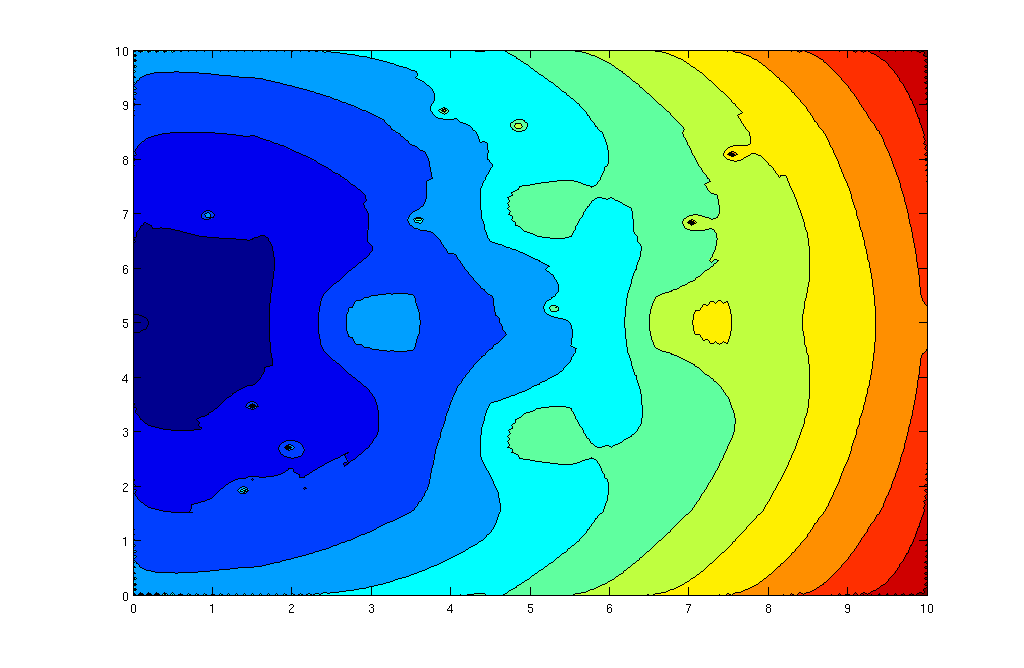
\includegraphics[width=0.8\textwidth]{../graphen/10agentsContour.png}
	\caption{Contour plot of room in figure \ref{emptyRoom} with 10 agents randomly positioned}
	\label{10agentsContour}
\end{figure}
\begin{figure}
	\centering
	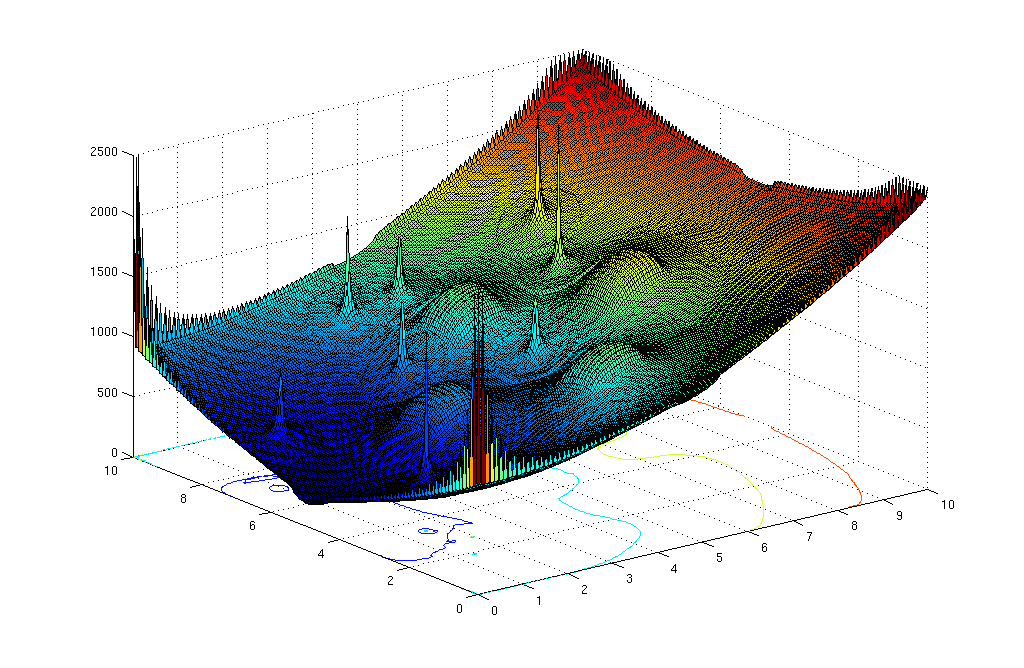
\includegraphics[width=0.8\textwidth]{../graphen/10agents3DPotential.png}
	\caption{3D of static potential field of the room in figure
	\ref{emptyRoom} with 10 agents randomly positioned}
	\label{10agents3D}
\end{figure}


\section{Exit Selection}
In emergency evcuation, the selection of the exit route is one of the most
important decisions. We take this into account in our simulation by the
implementation of the paper "Exit Selection with Best Response Dynamics"
\cite{BestResponseDynamics}. The paper describes an algorithm about how people
choose an appropriate exit based on the game theoretic concept of best
response dynamics. In the model the agents are the player and the strategies
are the possible target exits.

We assume that agents will select the fastest evacuation route. Despite of the
time related factor we include two other factors: familiarity and visibility
of the exits. The estimated evacuation time of an agent is the sum of the
estimated moving time and the estimated queueing time. The estimated moving
time is estimated simply by dividing the distance to the exit by the velocity
of the agent. The estimated queuing time depends on the exit's capacity and on
the number of the other agents that are heading towards the exit and are
closer to it than the agent itself. The estimated queuing time binds the
decision of a single agent to the decision of other agents. In conclusion,
this means the fastest exit route for a specific agent may change during the
evacuation.

The familiarity and visibility factor constrain the set of possible exits.
These factors can be seen as binary flags and the number of possible
combinations form the preference groups. Every door will be divided into a
preference group. Agents will select an exit from the nonempty group that has
the best preference. The doors in other preference groups are not of any
interest.

\subsection{Mathematical Formulation of the Model}
The agents are refered with indices $i$ and $j$, where $i,j \in \mathcal{N} =
\{1,2,3,...,N\}$. Exits can be seen as strategies, exits are denoted by $e_k,
k \in \mathcal{K} = \{1,2,...,K\}$. Strategies are denoted by $s_i \in
\{e_1,...,e_K\} = S_i, i \in \mathcal{N}$ where $S_i$ is a strategy set.

The agent's strategies are concluded by \[s := (s_{1},...,s_{N}) \in S_{1}
\times \cdot\cdot\cdot \times S_{N} = S \]  The strategies of all other agents
but agent $i$ is defined by \[s_{-i} := (s_{i},...,s_{i-1},s_{i+1},...,s_{N})
\in S_{-i}\] The estimated moving time depends on the agent $i$'s position
$\mathbf{r}_i$ and the exit $e_k$'s position $\mathbf{b}_k$. The positions of
the agents are in the set $\mathbf{r} := (\mathbf{r}_1,...,\mathbf{r}_N)$. So
the distance between agent $i$ and the exit $e_k$ is \[d(e_{k};\mathbf{r}_i) =
||\mathbf{r}_i - \mathbf{b}_k||\] The estimated moving time is the division of
the distance $d(e_{k};\mathbf{r}_i)$ by agent $i$'s velocity $v^{0}_i$
\[\tau_i(e_k;\mathbf{r}_i) = \frac{1}{v^{0}_i}d(e_k;\mathbf{r}_i)\] The
estimated queueing time is defined by the sum of all agents but agent $i$
heading towards exit $e_k$ and are closer to exit $e_k$ divided by the exit
$e_k$'s capacity $\beta_k$.

The subset of all agents $j \ne i$ who are closer to $e_k$ than agent $i$ is
given by \[\Lambda_i(e_k, s_{-i};\mathbf{r}) = \{j \ne i | s_j = e_k,
d(e_k;\mathbf{r}_j) \le d(e_k;\mathbf{r}_i)\}\] The number of elements in the
subset $\Lambda_i(e_k, s_{-i};\mathbf{r})$ is denoted by
\[\lambda_i(e_k,s_{-1};\mathbf{r}) = |\Lambda_i(e_k, s_{-i};\mathbf{r})| \]
The exit $e_k$'s capacity $\beta_k$ is a scalar value telling us how many
agents can pass the exit $e_k$ at once.

So the estimated queueing time is
\[\frac{1}{\beta_k}\lambda_i(e_k,s_{-1};\mathbf{r}) = |\Lambda_i(e_k, s_{-i};\mathbf{r})|\]
The sum of the estimated moving time and estimated queueing time gives us the
estimated evacuation time for agent $i$ through the exit $e_k$
\[T_i(s_i, s_{-i};\mathbf{r}) = \frac{1}{\beta_k}\lambda_i(e_k,s_{-1};\mathbf{r}) + \tau_i(e_k;\mathbf{r}_i)\]
As a result of the game theoretic principle, the strategy of agent $i$ is the
best response to the other agents' strategies. This means every agent will
choose the exit which has the lowest evacuation time.
\[s_i = BR_i(s_{-i};\mathbf{r}) = \arg \underset{s^{\prime}_i \in S_i}{\min} T_i(s^{\prime}_i,s_{-i};\mathbf{r}) \]
As we have mentioned before the effects of familiarity and visibility of exits
can constrain the group of possible exits for agent $i$, these conditions are
taken into account by defining two binary flags
\[fam_i(e_k),\ vis(e_k;\mathbf{r_i}),\quad \forall\ i \in \mathcal{N}, k \in K\]
The binary flags give certain information about agent $i$:
\[fam_i(e_k) \ = \ 
\begin{cases} 
1 & \text{if exit\ } e_k \text{\ is familiar to agent\ } i \\
0 & \text{if exit\ } e_k \text{\ is not familiar to agent\ } i
\end{cases}\]
\[vis(e_k; \mathbf{r}_i) = \ 
\begin{cases} 
1 & \text{if exit\ } e_k \text{\ is visible to agent\ } i \\
0 & \text{if exit\ } e_k \text{\ is not visible to agent\ } i
\end{cases}\]
These factors are the criterias for dividing the exits in to groups with
preference numbers. There are four possible combinations which means there are
four groups of exits with preference numbers from one to four. The smaller the
preference number is, the more preferable the exit. The familiarity of an exit
has a bigger influence about how preferable an exit is. Studies have shown
that evacuees prefere familiar routes even if there is a shorter route
\cite{BestResponseDynamics}. The visibility flag is important for the
calculation of the estimated queueing time beacause an agent is only able to
estimate the queue in front of a door if he can see the door.

According to the previous definition the doors will be grouped as shown in the table below.
\begin{center}
\begin{tabular*}{\textwidth}{@{\extracolsep{\fill}} cccc}
	\hline
	Preference number & Exit group &  $vis(e_k; \mathbf{r}_i)$ & $fam_i(e_k)$\\ 
	\hline

	1 & $E_i(1)$ & 1 & 1\\ 

	2 & $E_i(2)$ & 0 & 1\\ 

	3 & $E_i(3)$ & 1 & 0\\ 

	4 & No Preference & 0 & 0\\
	\hline
\end{tabular*}
\end{center}

\textbf{Table 1} The preference groups in which the exits will be divdided
into. The smaller the preference number, the more preferable the exit. The
fourth preference group describes people in panic which are not familiar with
the exits and can not see any either. \cite{BestResponseDynamics}

Mathematically the selection of the door is defined as
\[s_i = BR_i(s_{-i};\mathbf{r}) = \arg \underset{s^{\prime}_i \in S_i}{\min} T_i(s^{\prime}_i,s_{-i};\mathbf{r})\]
\[s^{\prime}_i \in E_i(\overline{z})\]
The specific agent $i$ chooses an exit from the non-empty Group
$E_i(\overline{z})$ which has the best preference number $\overline{z}$ for
him. 

In addition to the paper we added an extra patience factor. The patience
factor is a simple comparison between the evacuation time of the preferable
new exit and the previously chosen exit. This is needed because it may happen
that an exit in a better preference group gets in sight. Despite the fact that
the exit is in a better preference group the evacuation time could take much
longer. So the agent will not redecide if the evacuation time of the new
preferable exit is greater than the evacuation time of the agent's previous
decision. This could be omitted if the number of exits is significant higher
than the number of possible preference groups.






\section{Implementation}
The simulation is split into several function files. The main file, where the
whole simulation is running, is the \textit{simulation.m}. This file needs
some information of the room, the walls and doors, the agents and so on to
run. What it exactly needs, can be looked up in the comment of the file.
To run some different kinds of simulation, we provide with the code some
\textit{initX.m} ($X \in 1\ldots5$) which construct different examples of
rooms and place the people at random positions. For an example of a running
matlab script please have a look at the first element in appendix A.

\subsection{Time Integration}
For the time integration we do an simple explicit euler. This means that we
integrate according to the following scheme: 
\[v_{i+1} = v_i + \delta t \cdot a_i \]
\[x_{i+1} = x_i + \delta t \cdot v_{i+1}\]
The $a$ is calculated as it was shown in the introduction of this report: 
\[ a = \frac{\delta^2 x_p}{\delta t^2}  = \frac{1}{m} \left( - \sum^{N}_{q = 1, q \neq p}
\nabla_{x_p} V_{agent}(|x_p - x_q|) - \nabla_{x_p} V_{door}(|x_p - x_q|) 
- \sum^{W}_{q = 1} \nabla_{x_p} V_{wall}(|x_p - x_q|)\right)\]



\newpage
\section{Simulation Results and Discussion}
The basic configuration of the simulation consists of a square room with a
side length of ten units. There are three evenly spread exits, located on the
west side. The exits are all of the same width and a capacity of one agent
per timestep. The simulation has two scenarios, the first one is an empty room
without any obstacles and the second scenario uses the same room geometry but
there is a pile in the front of every door. The piles are modelled as square
blocks with a sidelength of one unit. They use the same repulsive force as the
wall does. (see figure \ref{rooms})

There are five cases with 100, 200, 300, 400 and 500 agents. Every test case
consists of twelve runs. The average of these twelve runs will be used in the
analysis.
\begin{figure}
	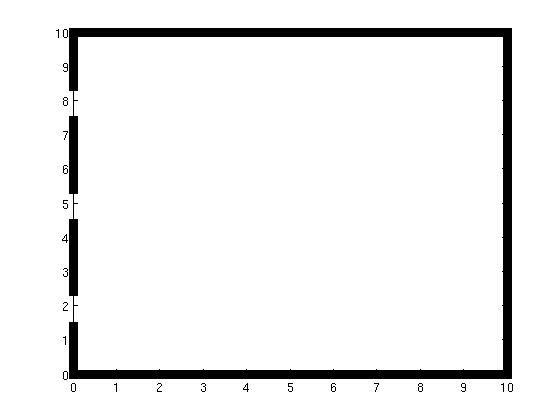
\includegraphics[width=0.5\textwidth]{../graphen/raum_ohne_piles.jpg}
	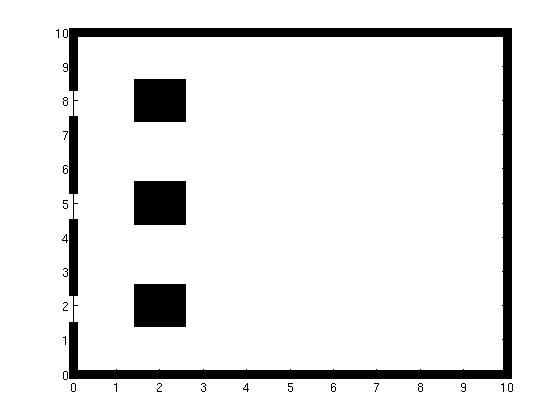
\includegraphics[width=0.5\textwidth]{../graphen/raum_mit_piles.jpg}
	\caption{The rooms with and without piles used in the simulation.}
	\label{rooms}
\end{figure}
\subsection{Exit Time Comparison}
We see some differences between the two room configurations. In the
configuration with the piles, it takes longer until the people start to
leave the room. We think the reason may be that everybody has a direct way
to the doors and the doors are visible to all if there are no piles. This
means if the door is in sight, the people can estimate the queueing time so 
they are able to choose the door with best response in the first place.
By having piles, the people only know the route to doors they are familiar to.
If people get behind the piles all doors are in the line of sight. This means
the possibilites of choosing an exit expands rapidly and the frequency of 
redicisions increases. An other explanation for the slower evacuation in
the pile scenario may be that the pressure on the doors is lower. This causes
a smaller force acting on the people which results in a slower evacuation.
In figure \ref{noPileTimes} and \ref{pileTimes} one can see the number of people in the room versus
the time.
\begin{figure}
	\centering
	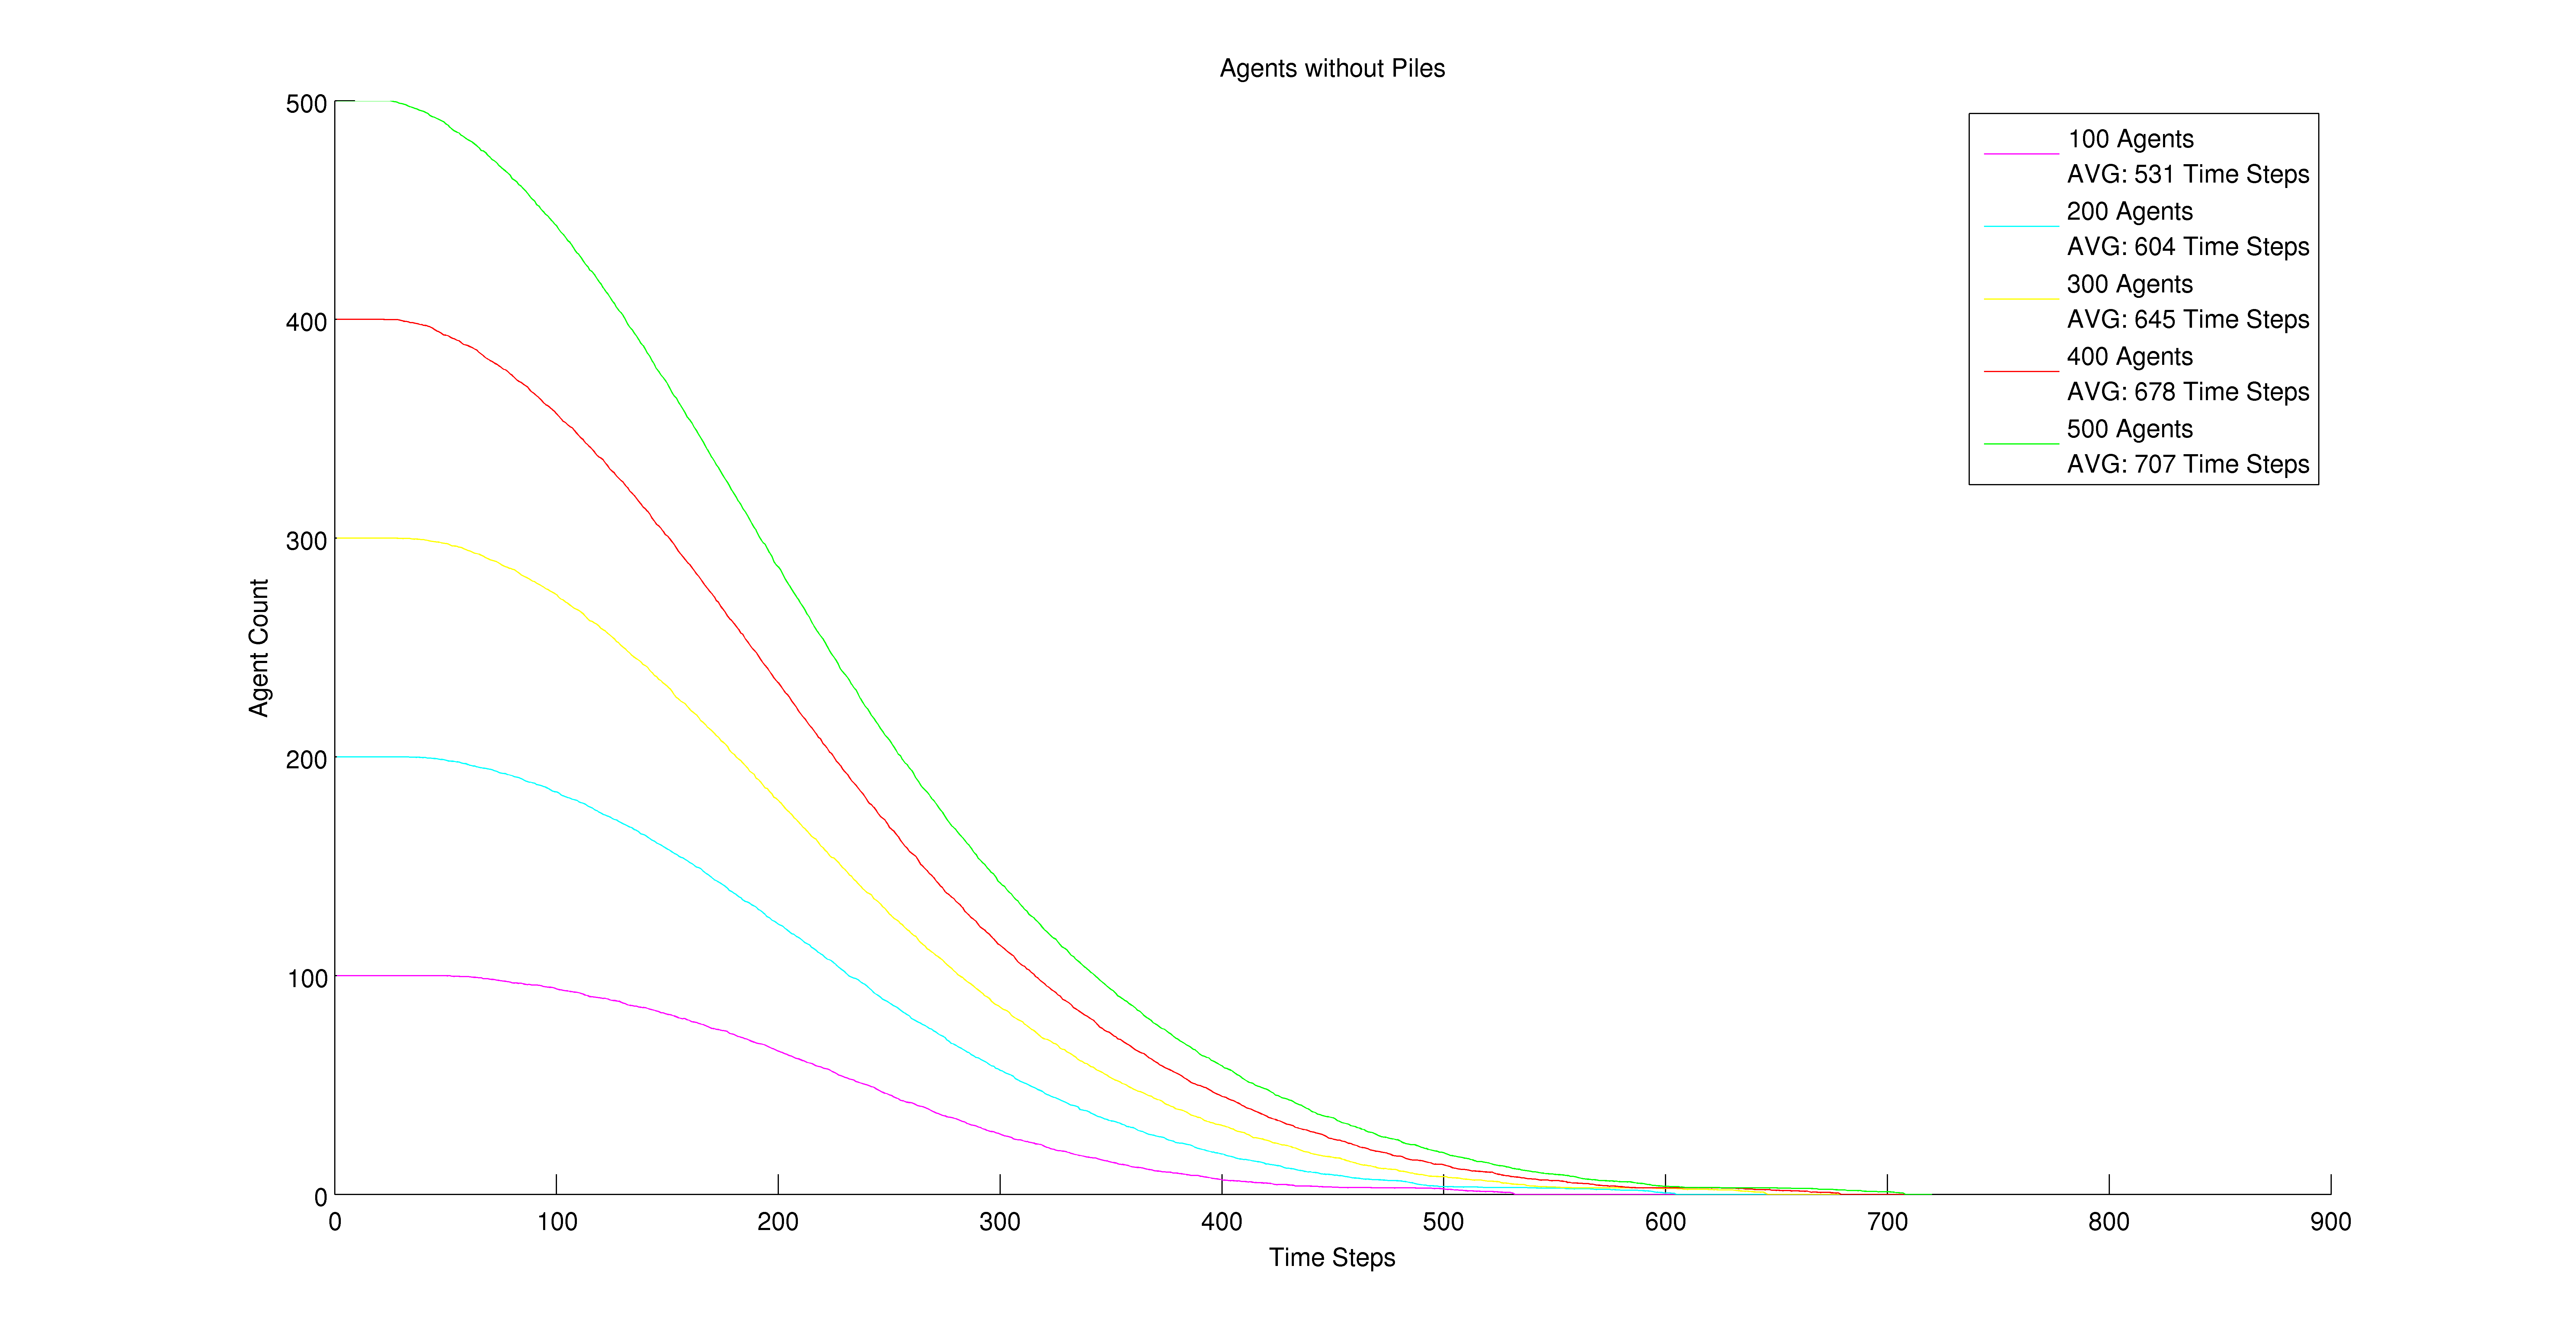
\includegraphics[width=0.9\textwidth]{../graphen/agents_ohne_piles.png}
	\caption{Exit times for different numbers of people in the room without
	piles}
	\label{noPileTimes}
\end{figure}
\begin{figure}
	\centering
	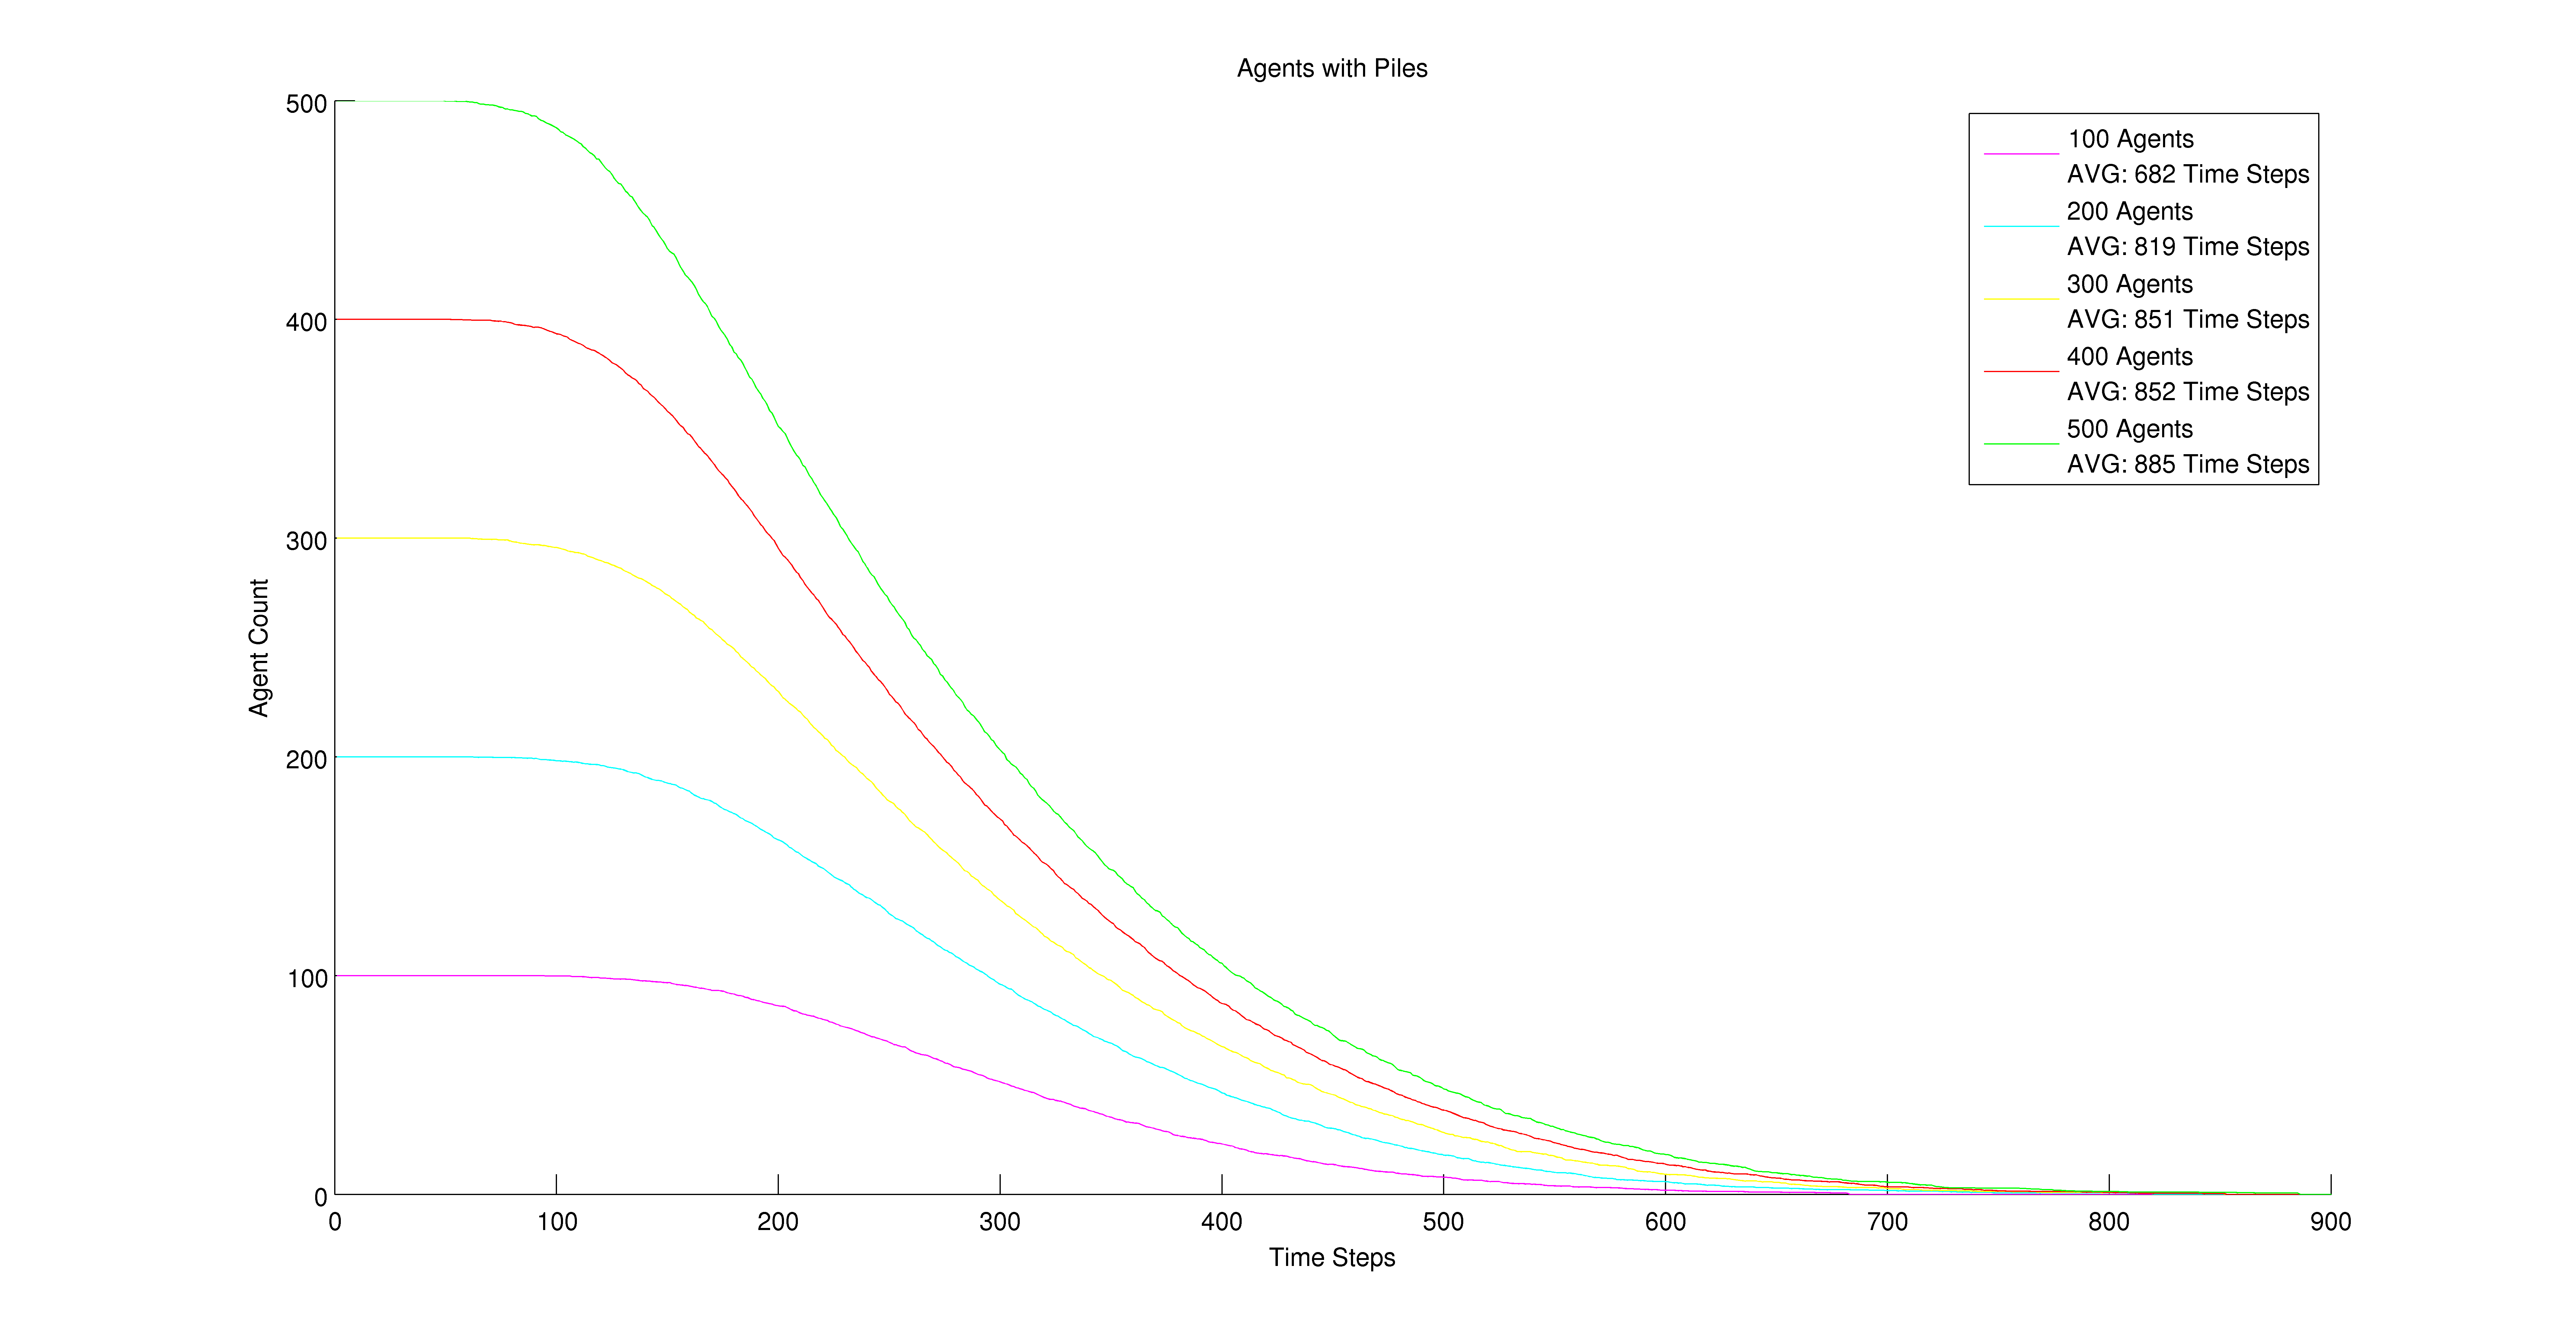
\includegraphics[width=0.9\textwidth]{../graphen/agents_mit_piles.png}
	\caption{Exit times for different numbers of people in the room with piles}
	\label{pileTimes}
\end{figure}
\subsection{Decisions}
We also have some plots were one can see, how many people changed their mind
per timestep. Here we can see a big difference between the two room
configurations. When we have piles, the number of people changing the door is
much smaller then without the piles but it goes much longer until we have a
small number of redecisions (figure \ref{noPileDecision} and \ref{pileDecision}).
We think this makes perfectly sense, since due to the exit selection we
implemented, a person which does not know something about a door and does not
see it, would not go to that door even if it was nearest. We think this is how
people would act in reality too.
\begin{figure}
	\centering
	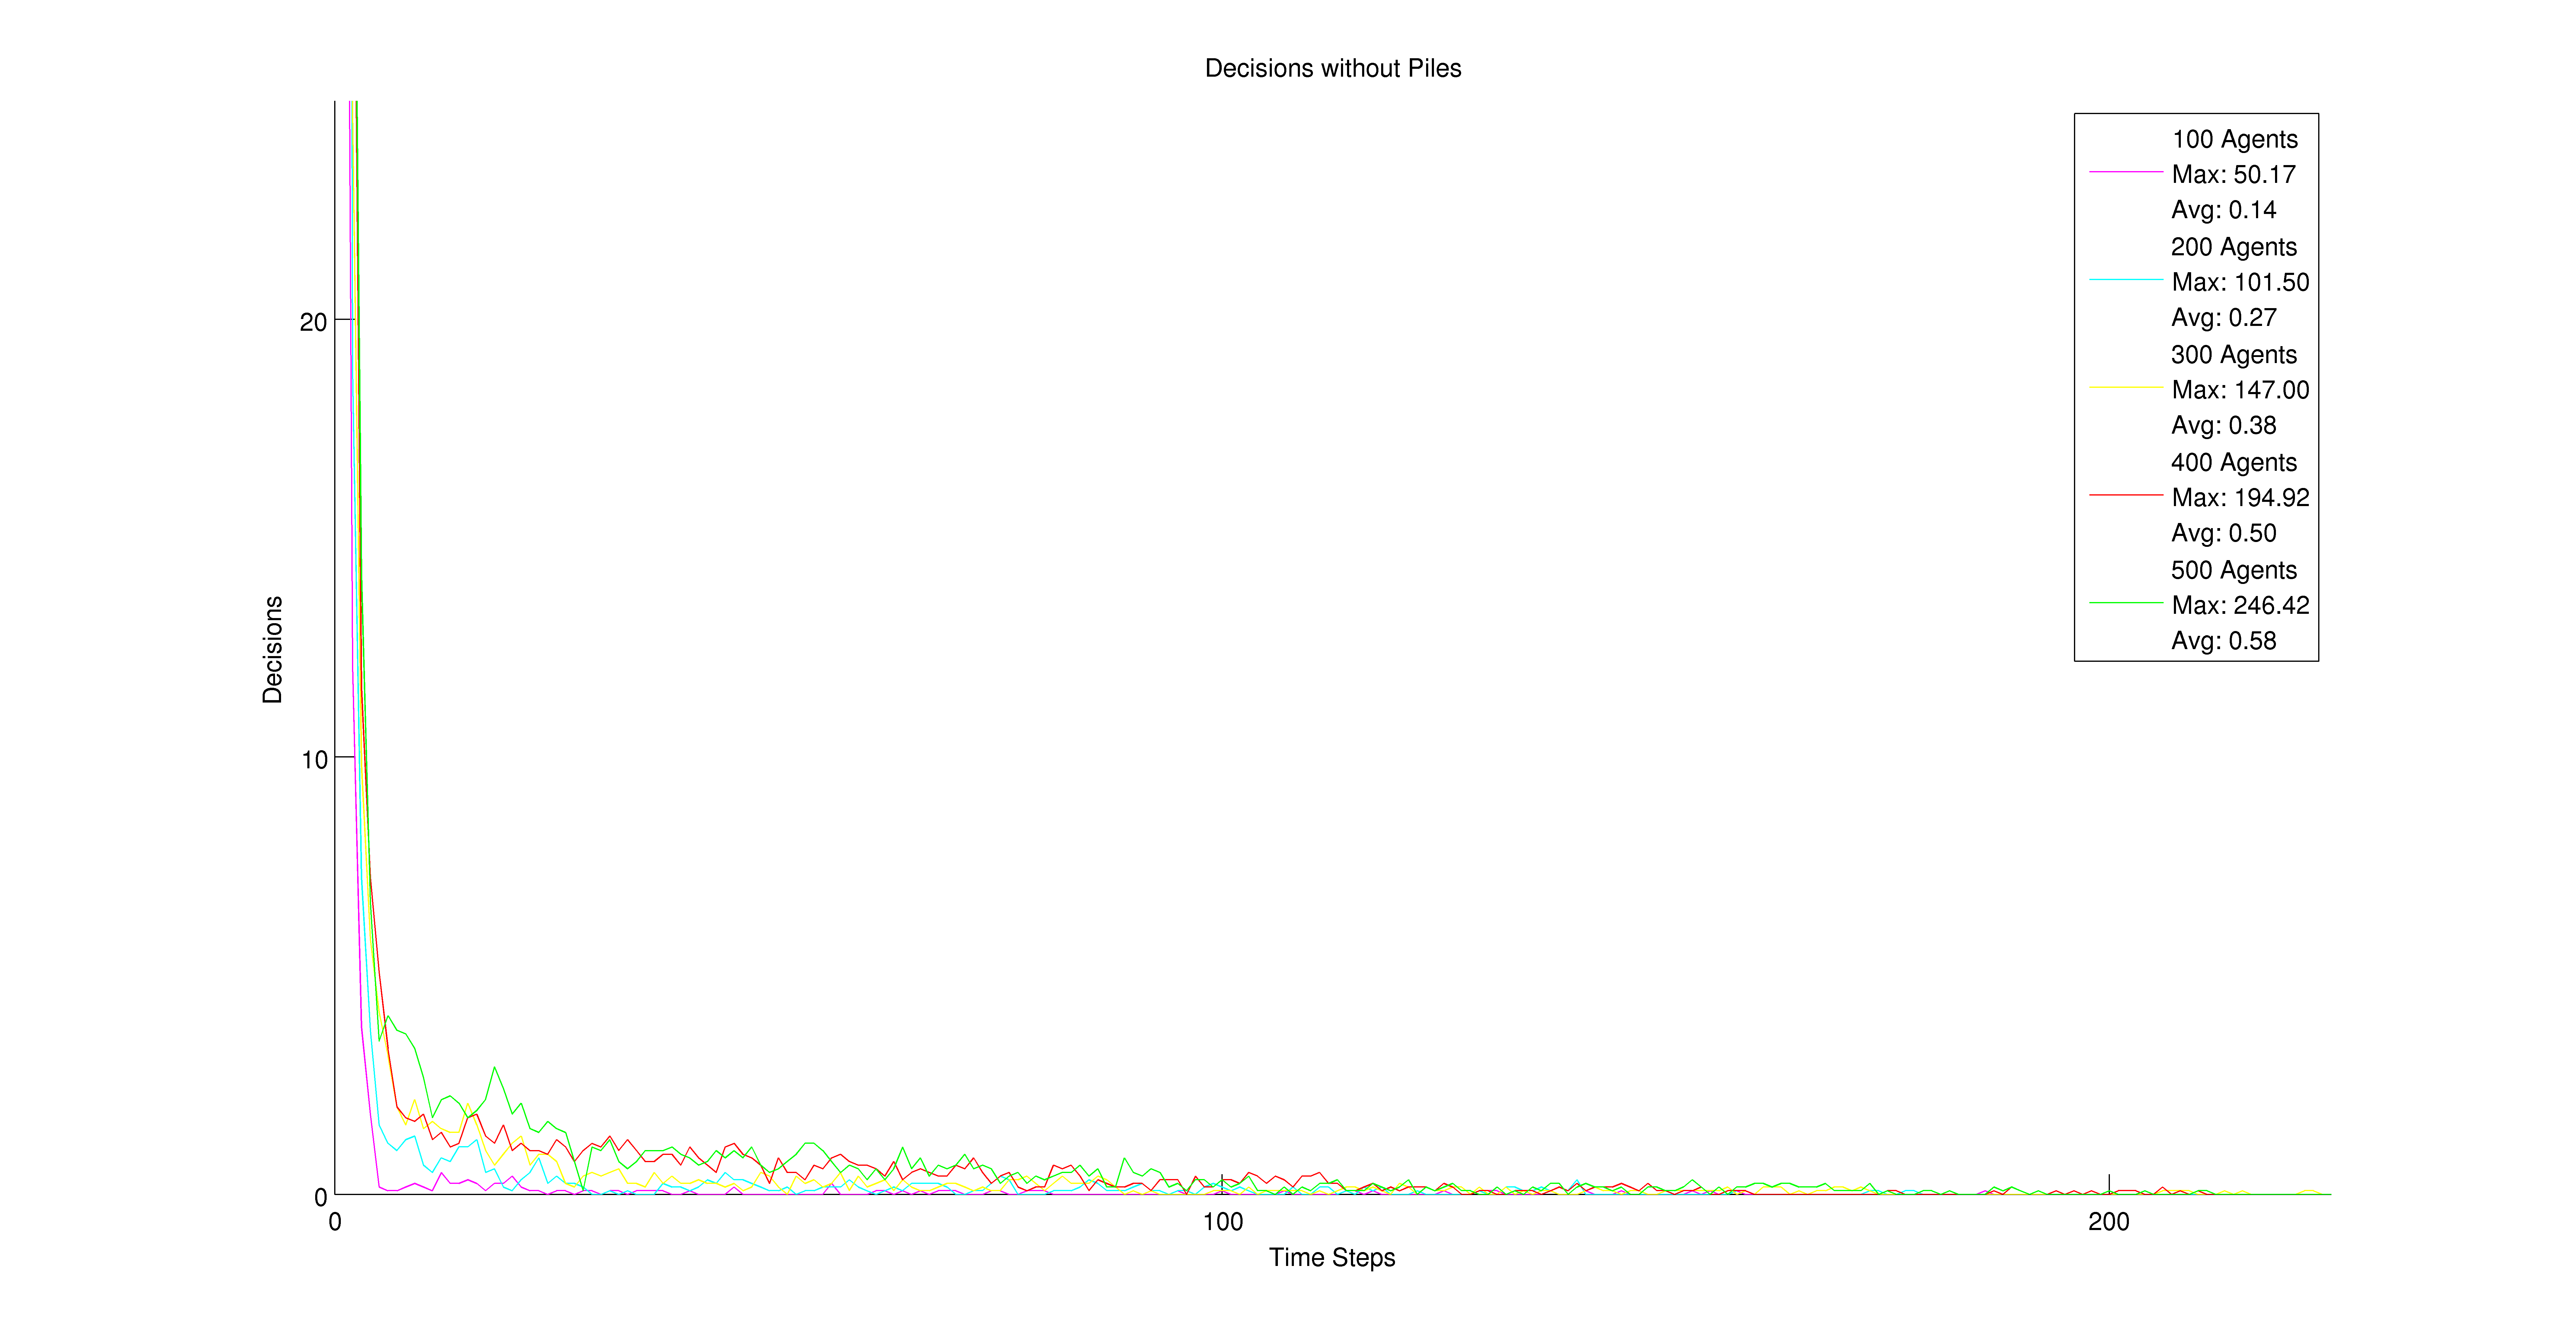
\includegraphics[width=0.9\textwidth]{../graphen/decisions_ohne_piles_2.png}
	\caption{Number of redecisions of persons in the room without piles}
	\label{noPileDecision}
\end{figure}
\begin{figure}
	\centering
	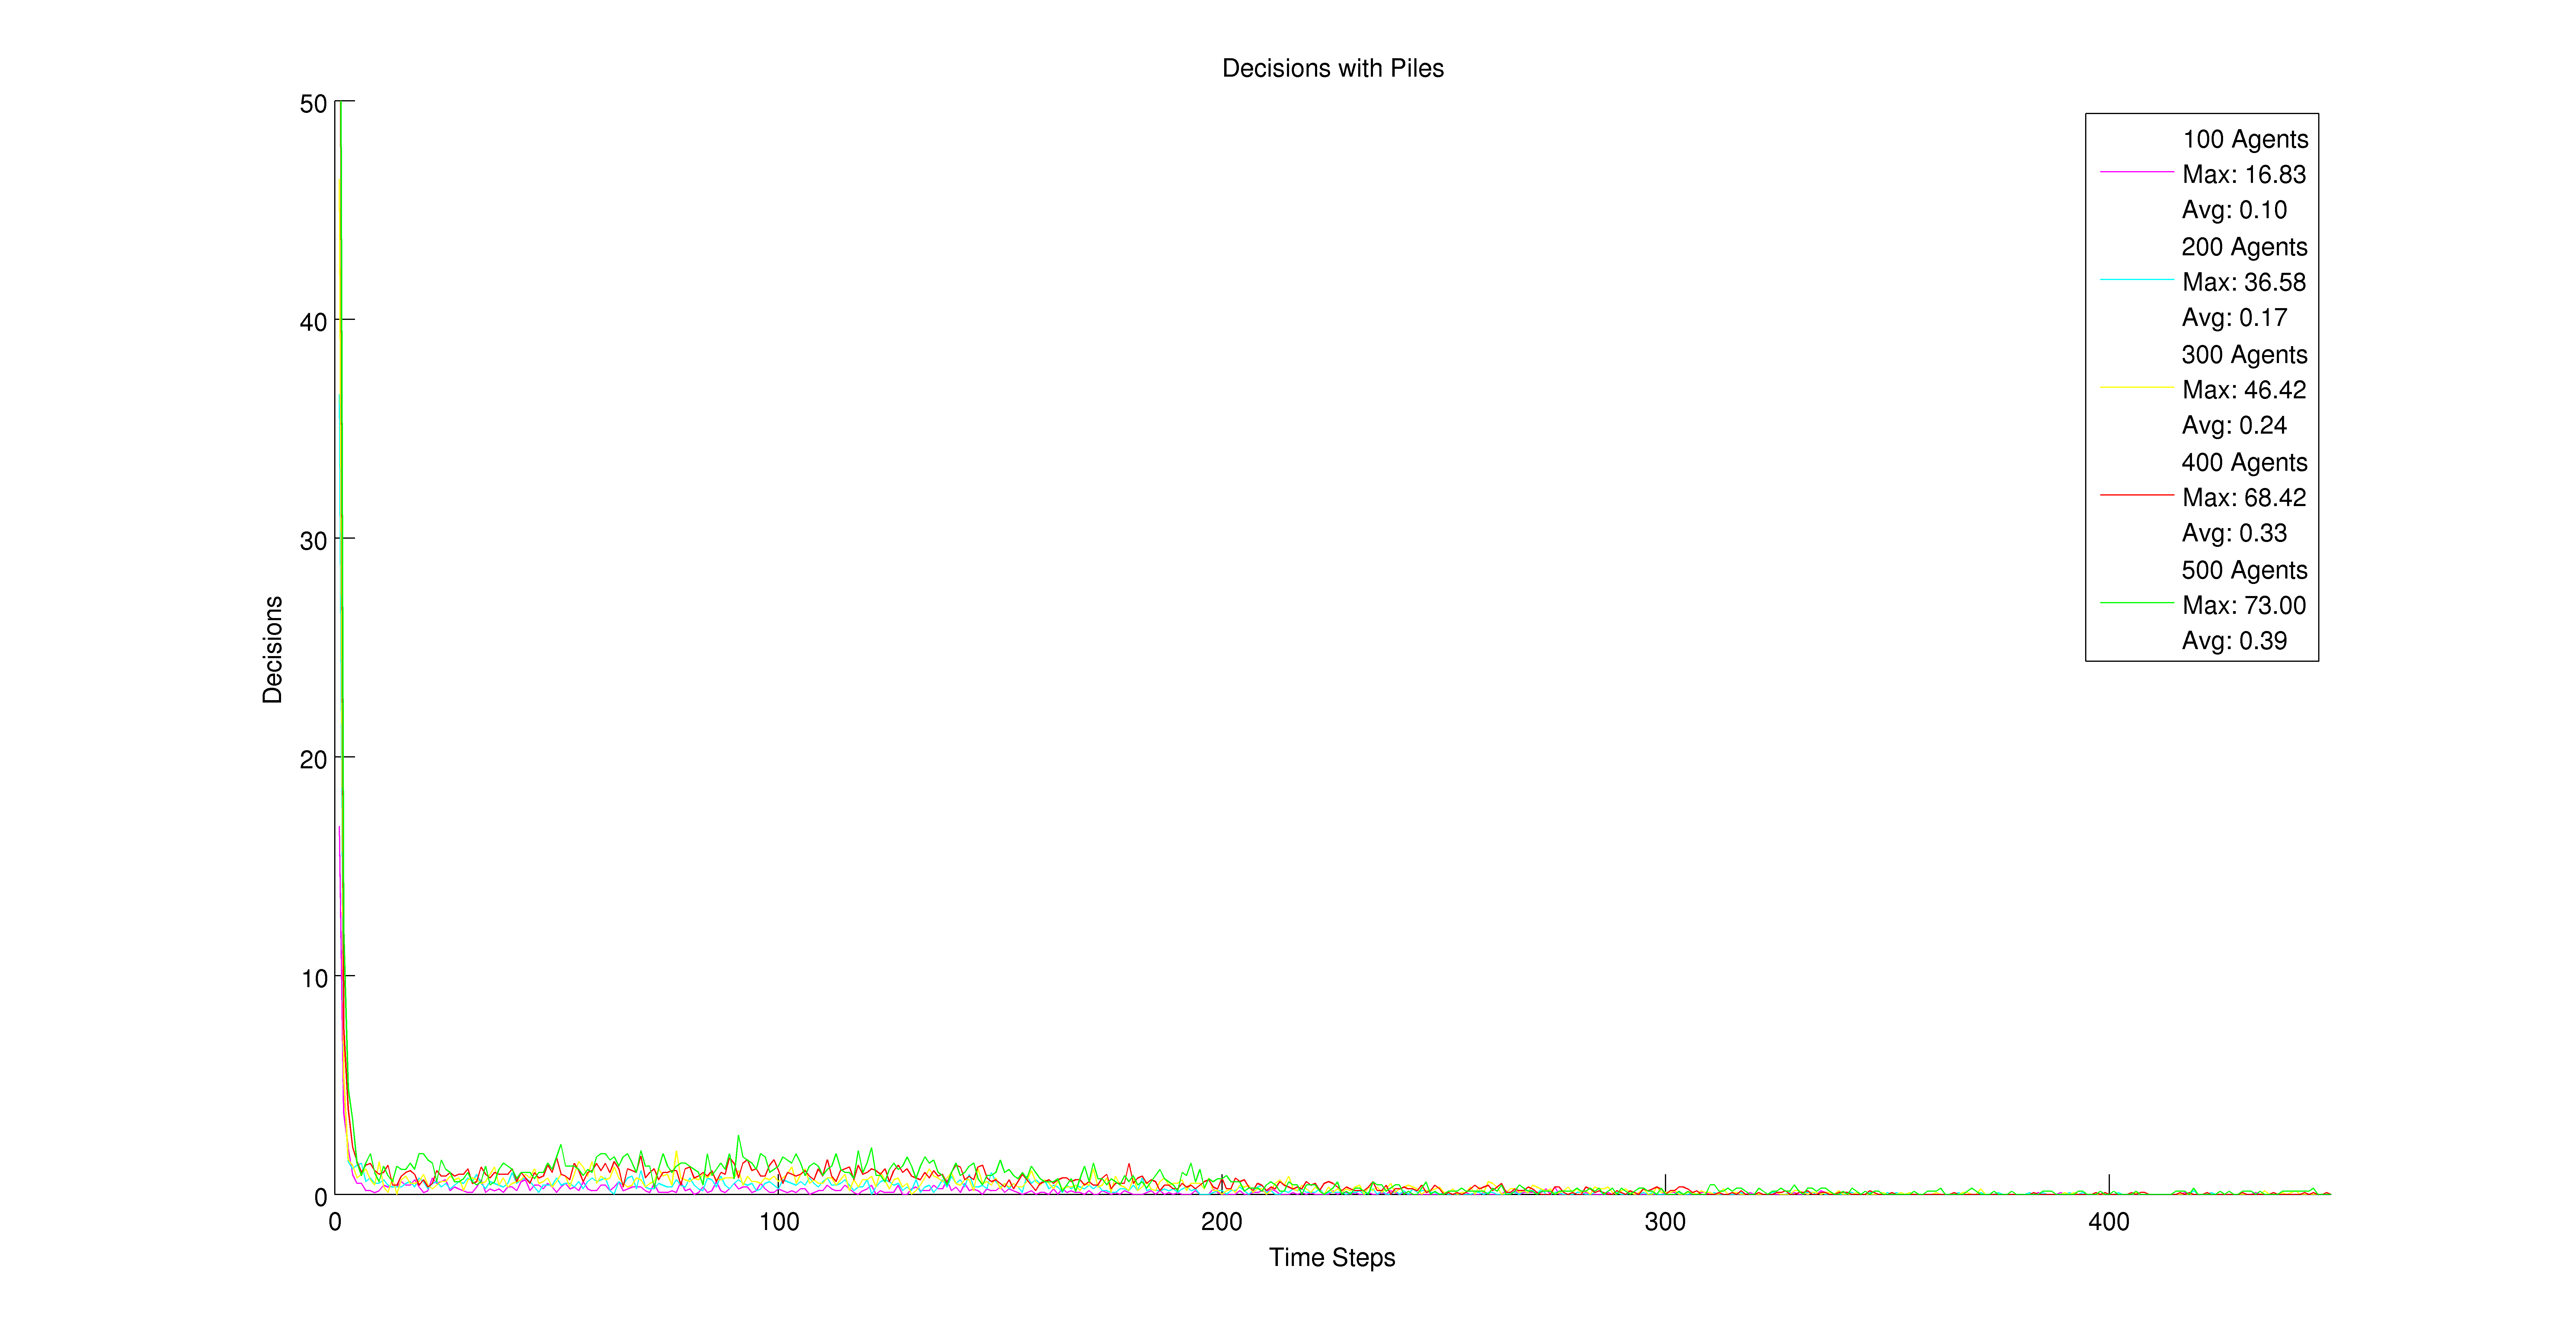
\includegraphics[width=0.9\textwidth]{../graphen/decisions_mit_piles_2.png}
	\caption{Number of redecisions of persons in the room with piles}
	\label{pileDecision}
\end{figure}

\newpage
\section{Summary and Outlook}
A continuous model for evacuation scenarios was implemented. By running the
software, we get some charactersitics of the crowd, which also happen in
reality. Additionally, the choosing of the door was done by best response
dynamics. Which is a game theoretical approach. 
The implemented model shows crowd characteristics, such as the circular form of the
crowd in front of a door, the redecition of the preferred door of people in
the crowd and more.

For further work, one could possibly implement the model with different
potential fields instead of the ones used. Also one could extend the static
fields in such a way, that the geometry can be more complex then it is in our
cases.

As a comparison, one could take the results from social experiments \cite{LianaManukyan} for
choosing the door and look if they give the same result. One example of such
an experiment gave the following evacuation strategies:
\begin{enumerate}
	\item I escaped according to the signs and instructions, and also
	broadcast or guide by shop-girls (46.7\%). 
	\item I chose the opposite direction to the smoking area to escape from
	the fire as soon as possible (26.3\%).
	\item I used the door because it was the nearest one (16.7\%).
	\item I just followed the other persons (3.0\%).
	\item I avoided the direction where many other persons go (3.0\%).
	\item There was a big window near the door and you could see outside. It
	was the most "bright" door, so I used it (2.3\%).
	\item I chose the door which I am used to (1.7\%).
\end{enumerate}



\newpage
\begin{thebibliography}{20}
\bibitem{ExtendedFloorField} K. Nishinari, A. Kirchner, A. Namazi and A. Schadschneider. 'Extended
floor field CA model for evacuation dynamics.' IEICE Trans Inf Syst (Inst
Electron Inf Commun Eng) VOL.E87-D;NO.3 (2006) pp(726-732).

\bibitem{FrictionEffects} A. Kirchner, K. Nishinari and A. Schadschneider. 'Friction effects
and clogging in a cellular automaton model for pedestrian dynamics.' PHYSICAL
REVIEW E67 056122(2003)

\bibitem{AnalyticalApprocach} D. Helbing, A. Johansson, J. Mathiesen, M. H. Jensen, and A. Hansen.
'Analytical Approach to Continuous and Intermittent Bottleneck Flows.'
PHYSICAL REVIEW LETTERS PRL 97 168001 (2006)

\bibitem{Centrifugal} W. J. Yu, R. Chen, L. Y. Dong, and S. Q. Dai. 'Centrifugal force
model for pedestrian dynamics'. PHYSICAL REVIEW E72 026112 (2005)

\bibitem{Dynamical}Takashi Nagatani 'Dynamical transition and scaling in a mean-field
model of pedestrian flow at a bottleneck' Physica A 300 (2001) pp(558-566)

\bibitem{BestResponseDynamics} Harri Ehtamo , Simo Heli\"ovaara1 , Simo
Hostikka , Timo Korhonen. 'Modeling Evacuees Exit Selection with Best
Response Dynamics'. Fire Safety Journal, Volume 41, Issue 5, July 2006, Pages 364-369

\bibitem{InternalObstacles} Hai-Jun Huang, Ren-Yong Guo. 'Static Floor Field and
exit choice for pedestrian evacuation in rooms with internal obstacles
and multiple exits'. Phys. Rev. E 78, 021131 (2008)

\bibitem{CollectivePenomena} Andreas Schadschneider , Ansgar Kirchner ,
Katsuhiro Nishinari. 'CA Approach to Collective Phenomena in
Pedestrian Dynamics'. Lecture Notes In Computer Science; Vol. 2493 (2002)
pp(239-248)

\bibitem{LianaManukyan} Liana Manukyan, 'Evacuation Bottleneck', 
Modelling and Simulating Social Systems with MATLAB, ETH Zurich, December 2009
\end{thebibliography}
\newpage
\begin{center}
	\LARGE Appendix A: Matlab Code
\end{center}

\lstinputlisting{../code/main.m}
\lstinputlisting{../code/debug.m}
\lstinputlisting{../code/simulation.m}
\lstinputlisting{../code/force.m}
\lstinputlisting{../code/basic2.m}
\lstinputlisting{../code/potAgent.m}
\lstinputlisting{../code/potWall.m}
\lstinputlisting{../code/potDoor.m}
\lstinputlisting{../code/distance_time.m}
\lstinputlisting{../code/get_queue_count.m}
\lstinputlisting{../code/is_vis.m}
\lstinputlisting{../code/is_fam.m}
\lstinputlisting{../code/init1.m}
\lstinputlisting{../code/init2.m}
\lstinputlisting{../code/init3.m}
\lstinputlisting{../code/init4.m}
\lstinputlisting{../code/init5.m}
\lstinputlisting{../code/plotField.m}
\lstinputlisting{../code/plotStats.m}

%\newpage
%\begin{center}
%	\LARGE Appendix B: Leveleditor
%\end{center}
%\Large index.html
%\verbatiminput{../leveleditor/index.html}
%\Large script.js
%\verbatiminput{../leveleditor/script.js}

\end{document}  



 
